\section{System Architecture}
\label{sec:system_architecture}

The CFI-Care system is built upon a robust three-tier architecture designed to
facilitate secure and interoperable healthcare data management. The system
integrates a modern frontend, a logic-heavy middleware layer, and a
standards-compliant backend to ensure data consistency and security. The
architecture adheres to the FHIR (Fast Healthcare Interoperability Resources)
standard for all medical data exchange and utilizes OAuth 2.0 via Keycloak for
identity management.

\subsection{High-Level Architecture}

The application operates through a strict separation of concerns. The
Presentation Layer is an Angular-based Single Page Application (SPA) that
serves as the user interface. It does not communicate directly with the data
stores. Instead, all client requests are intercepted by an Nginx Reverse Proxy,
which handles SSL/TLS termination and routes traffic to the appropriate
internal services.

The core of the backend processing is handled by the Node.js Application
Server. This server acts as the primary API gateway, implementing business
logic, enforcing security policies, and managing user sessions. It communicates
with the HAPI FHIR Server, a specialized Java-based component responsible for
persisting clinical data in compliance with the FHIR R5 standard. Data storage
is consolidated in PostgreSQL databases, while high-speed data access and
session management are handled by Redis instances.

\begin{figure}[H]
    \centering
    \fbox{\begin{minipage}[c][12cm]{\textwidth}
            \centering
            % \vspace{5cm}
            \includegraphics[width=0.95\textwidth]{Backend/Images/SystemArchitecture.drawio.png}
        \end{minipage}}
    \caption{High-Level Container Architecture showing the interaction between the Nginx proxy, application services, and data persistence layers.}
    \label{fig:high_level_arch}
\end{figure}

\subsection{Node.js Application Server}

The Node.js server, built with the Express.js framework, serves as the
middleware layer that bridges the gap between the user interface and the
standardized medical records. It is designed with a modular layered
architecture to ensure scalability and maintainability.

\subsubsection{Middleware and Security}
Upon receiving a request, the server passes it through a comprehensive
middleware stack. Security headers are applied using Helmet to prevent common
web vulnerabilities. Cross-Origin Resource Sharing (CORS) is configured to
restrict access to authorized domains. Crucially, the server implements rate
limiting to protect API endpoints from abuse and utilizes a Redis-backed
session store to manage user authentication states efficiently.

\subsubsection{Routing and Services}
The application is divided into specific route modules corresponding to
healthcare domains. Dedicated endpoints manage Patients, Practitioners,
Encounters, and Episodes of Care. A specialized "History Graph" module handles
the retrieval and processing of graph visualization data.

Beneath the routing layer lies the service layer, which contains the core
business logic. These services act as proxies to the FHIR server, transforming
raw FHIR JSON into formats optimized for the frontend, such as the D3.js
visualizations. They also handle document processing tasks, such as converting
base64 strings to PDF files for binary storage.

\begin{figure}[H]
    \centering
    \fbox{\begin{minipage}[c][12cm]{\textwidth}
            \centering
            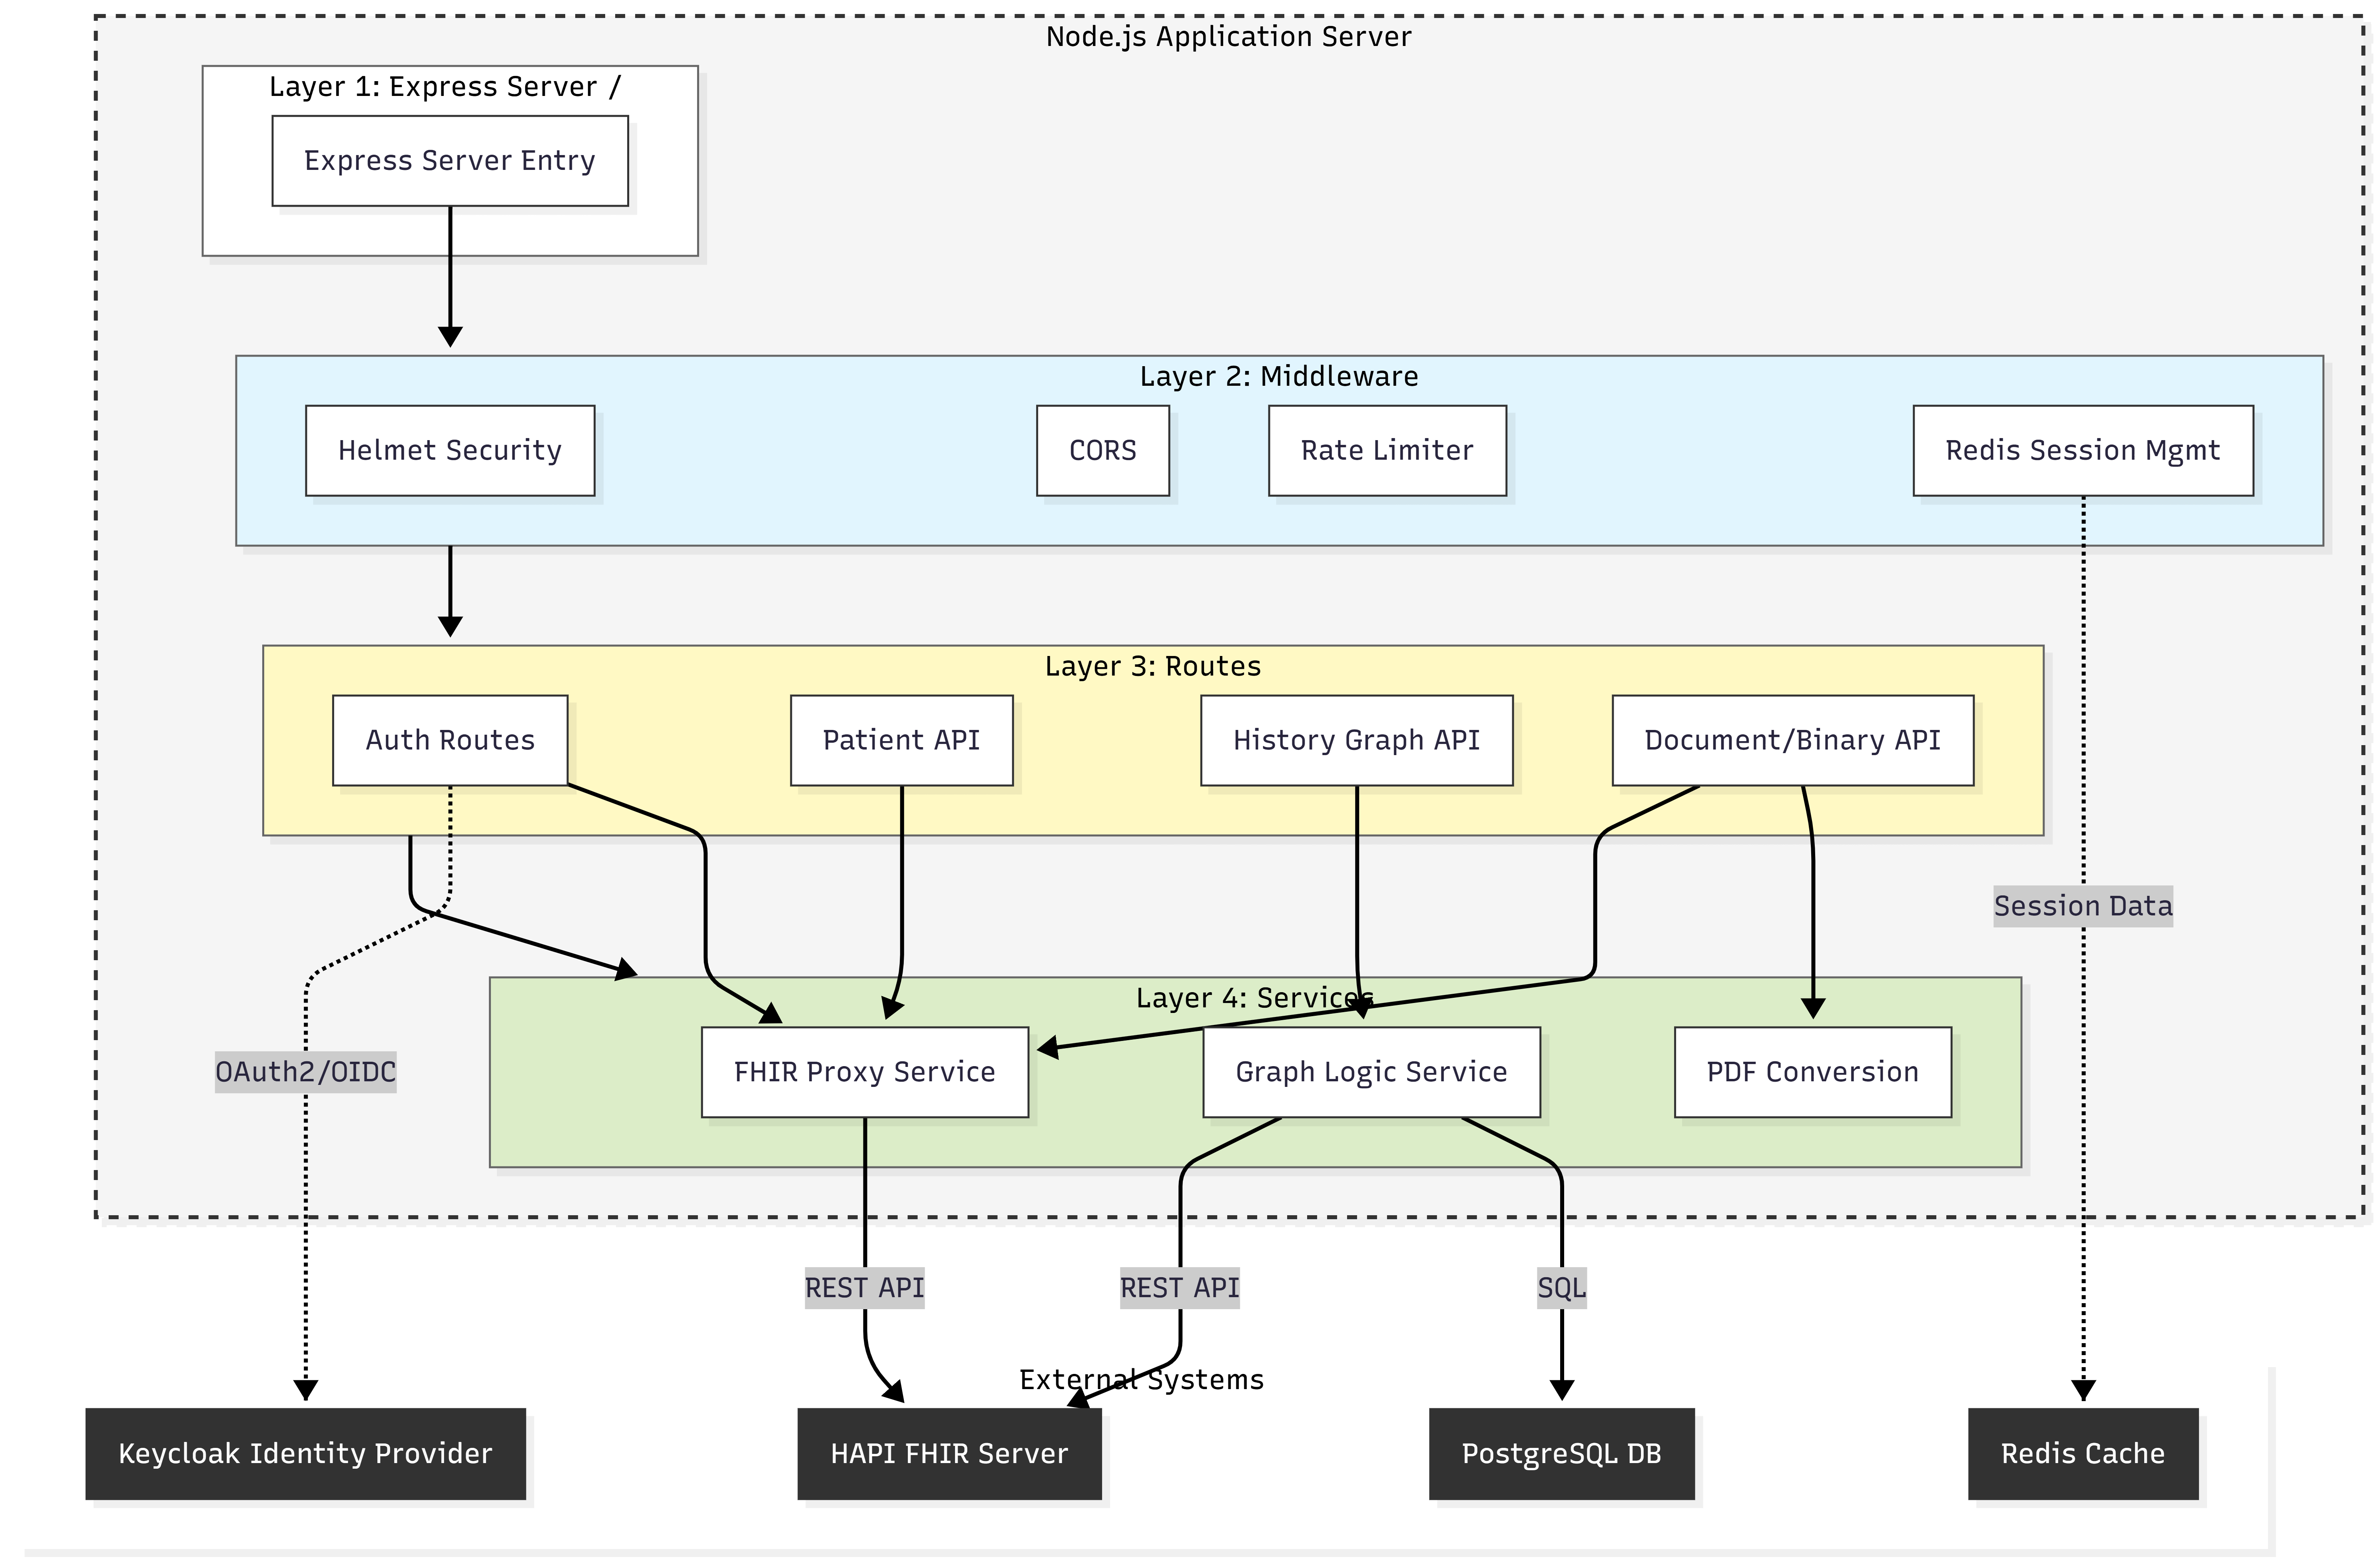
\includegraphics[width=0.95\textwidth]{Backend/Images/InternalNodeJsArch.png}
        \end{minipage}}
    \caption{Internal layered architecture of the Node.js Application Server, detailing the middleware stack and service distribution.}
    \label{fig:nodejs_layers}
\end{figure}

\subsection{Data Persistence and Schema}

The system utilizes a polyglot persistence strategy, employing different
database technologies for specific use cases to maximize performance.

\subsubsection{Relational Data}
The primary storage engine is PostgreSQL. It is divided into two logical
segments. The first segment supports the HAPI FHIR server, storing all standard
clinical resources (like Patients and Observations) in a highly structured
format managed by Hibernate. The second segment supports the Keycloak identity
provider, storing user credentials and realm configurations.

\subsubsection{Custom Graph Schema}
To support the unique "Medical History Graph" feature, a custom schema was
designed alongside the standard FHIR tables. This schema consists of
\texttt{encounter\_nodes} and \texttt{node\_relations}. These tables allow the
system to map standard FHIR Encounters into a Directed Acyclic Graph (DAG),
enabling the visualization of a patient's journey through time with causal
links between medical events.

\subsubsection{Caching and Auditing}
Redis is utilized for ephemeral data storage. One instance is dedicated to
storing user sessions, ensuring fast authentication checks. A second Redis
instance operates in Append-Only File (AOF) mode to store audit logs, providing
a persistent and high-speed trail of system activities.

\begin{figure}[H]
    \centering
    \fbox{\begin{minipage}[c][12cm]{\textwidth}
            \centering
            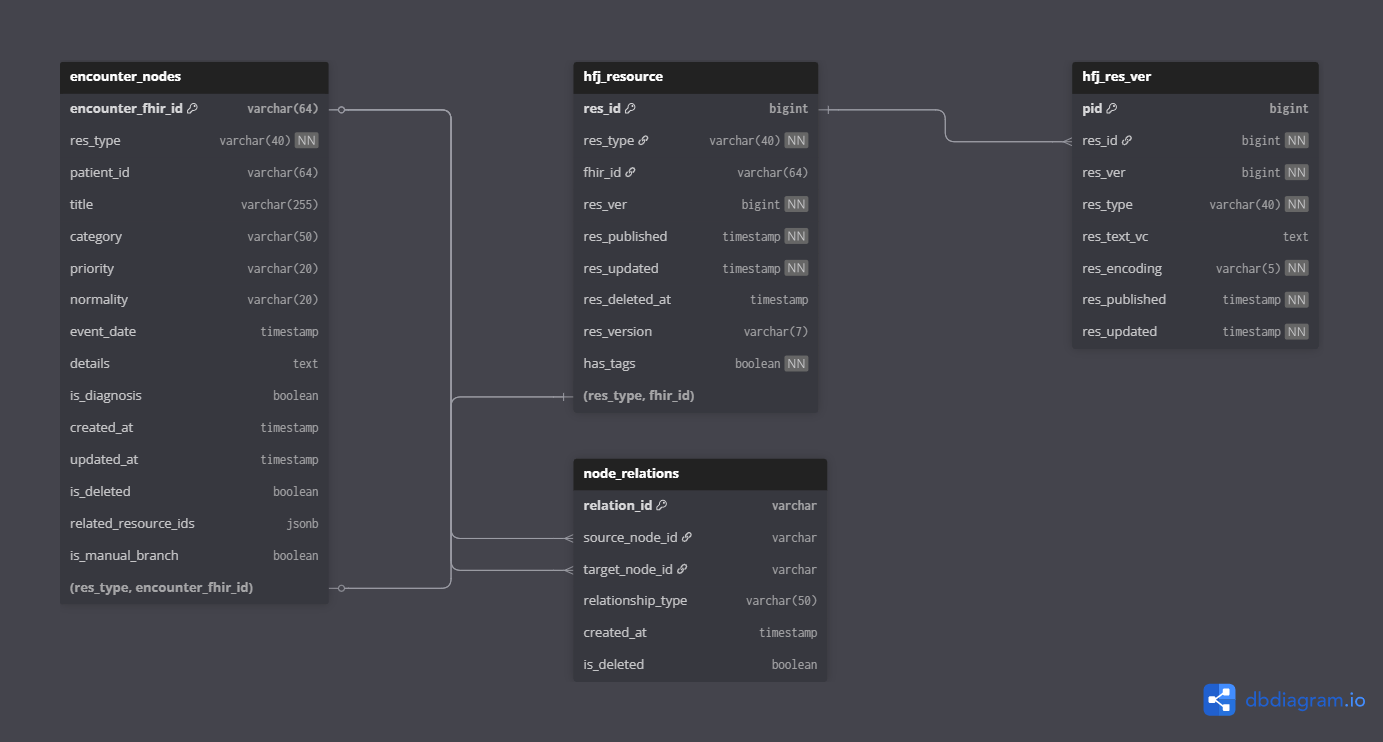
\includegraphics[width=1\textwidth]{Backend/Images/PatientsDatabaseSchema.png}
        \end{minipage}}
    \caption{Entity-Relationship Diagram (ERD) illustrating the integration of custom graph tables with the standard FHIR resource table.}
    \label{fig:database_schema}
\end{figure}

\subsection{Security and Infrastructure Layer}

The infrastructure is secured through a centralized Identity and Access
Management (IAM) system using Keycloak. Keycloak handles all OAuth 2.0 and
OpenID Connect flows, issuing JSON Web Tokens (JWT) that the Node.js backend
validates against a public key set (JWKS).

All components are containerized using Docker and orchestrated via Docker
Compose. The environment is isolated within a private bridge network, with
Nginx acting as the sole entry point. Nginx enforces SSL/TLS encryption using
locally generated certificates, ensuring that all data in transit is encrypted.
Containers are configured with read-only file system mounts and strict
privilege limitations to minimize the security attack surface.